% ============================================================================
\section{Where the Gain Comes From}
\label{sec:regime}

Table~\ref{tab:generated} and Figure~\ref{fig:generated} report generated-answer
effects under the three data regimes with the frozen configuration (empirical Bayes,
$\kappa=2$, Team$\cap$Class, absolute scaling). Blind feedback costs $-0.0444$
$[-0.0606,-0.0285]$ when procedures overlap and becomes indistinguishable from zero
under strict disjointness ($+0.0008$ $[-0.0063,+0.0084]$, $p=.86$). The direct
protocol contrast falls from $+0.0549$ $[+0.0389,+0.0710]$ on the familiar panel to
$+0.0085$ $[+0.0016,+0.0158]$ on the strict panel. The conditioned effect is small
in every regime ($+0.0093$ to $+0.0149$); on the strict panel its cosine interval
excludes zero while the rank test is marginal ($p=.066$), ROUGE-L is not
significant, and the estimate lies below the study's 80\,\% MDE (0.0103). We
therefore describe it as a small, metric-dependent effect, not as a confirmed gain.

\Table[!btp](width=\textwidth){Generated-answer cosine difference against the
no-feedback baseline (paired, per ticket) under three data regimes and three
evidence sources. Brackets are 95\,\% ticket-level paired bootstrap intervals. The
finalist is empirical Bayes with $\kappa=2$, Team$\cap$Class scope and absolute
scaling. The direct contrast is shown in Figure~\ref{fig:generated}b. Wilcoxon $p$
for conditioned/blind: familiar .029/.00015, duplicate .002/.655, strict
.066/.856. Holm-adjusted $p$ within the primary family: familiar .117/.001,
duplicate .011/1.000, strict .197/1.000.\label{tab:generated}}{
\begin{tabular}{@{}lrrrr@{}}
\toprule
Regime & $n$ & Conditioned & Blind & Reply similarity \\
\midrule
Familiar  & 398 & $+0.0105$ $[+0.0005, +0.0212]$ & $-0.0444$ $[-0.0606, -0.0285]$ & $+0.0143$ $[+0.0047, +0.0242]$ \\
Duplicate & 398 & $+0.0149$ $[+0.0059, +0.0246]$ & $-0.0214$ $[-0.0367, -0.0073]$ & $+0.0081$ $[+0.0016, +0.0152]$ \\
Strict    & 427 & $+0.0093$ $[+0.0026, +0.0169]$ & $+0.0008$ $[-0.0063, +0.0084]$ & $+0.0026$ $[-0.0039, +0.0097]$ \\
\bottomrule
\end{tabular}}

\begin{figure*}[!t]
\centering
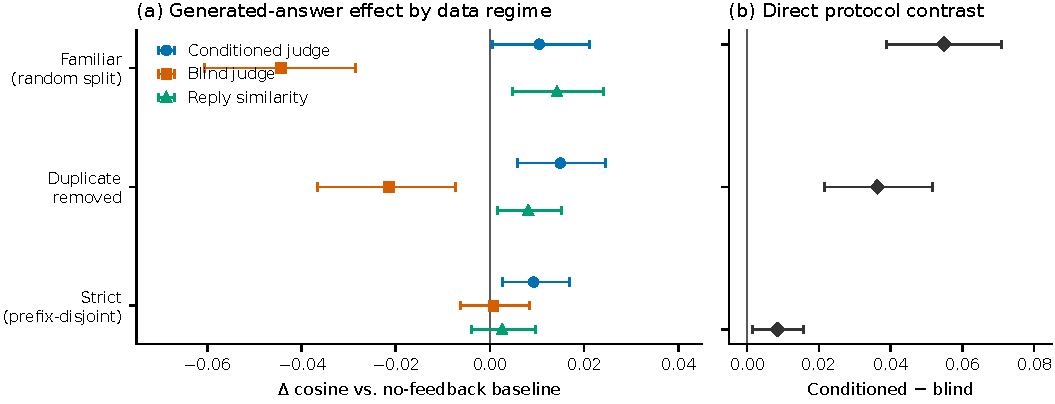
\includegraphics[width=\textwidth]{revision_ieee_access/03_manuscript/figures/fig2_generated_effects.pdf}
\caption{Generated-answer effects by data regime. (a)~Mean $\Delta$ cosine against
the no-feedback baseline for conditioned, blind and reply-similarity evidence; bars
are 95\,\% ticket-level paired bootstrap intervals. (b)~Direct conditioned-minus-blind
contrast on the same tickets. The blind harm on the familiar panel disappears on
the strict panel, while the conditioned effect remains small.}
\label{fig:generated}
\end{figure*}

The reply-similarity baseline, which uses no LLM judge, is competitive only where
procedure overlap remains. On the familiar panel it is at least as large as the
conditioned judge ($+0.0143$ versus $+0.0105$); on the duplicate panel it is
smaller ($+0.0081$ versus $+0.0149$); on the strict panel it is $+0.0026$ with an
interval that includes zero, against $+0.0093$ for the conditioned judge. The
ordering is consistent with the overlap explanation: a simple similarity prior can
recover part of the benefit when evaluation tickets share procedures or templates
with history, but it does not replace the judge when they do not.

Three families were fixed before adjustment (conditioned and blind across panels;
reply similarity; protocol contrast) and Holm-corrected within family. Blind harm
on the familiar panel survives ($p=.0009$); the conditioned effect on the familiar
panel does not ($p=.1165$); the duplicate conditioned effect does ($p=.0106$); the
strict conditioned effect does not ($p=.1965$). The strict protocol contrast
survives ($p=.0322$) but lies below its 80\,\% MDE (0.0101). The design is not
powered to estimate an effect of that size precisely; we report it as small and
imprecisely estimated, not as evidence of absence.

At retrieval level the same pattern appears more strongly. The legacy Laplace
conditioned top-1 proxy falls from $+0.034$ on the familiar panel to $+0.002$ on
the strict panel and is significant in 0 of 5 group-aware splits; the calibrated
lift keeps a small positive point estimate ($+0.009$, 2 of 5 splits). The retrieval
proxy ranks configurations correctly but does not certify significance; the
generated intervals and the expert assessment do. This is why every claim in the
article is computed from generated answers, and the proxy is used only to select
configurations cheaply.

The interpretation is deliberately narrow. The familiar-panel conditioned gain is
not evidence that the judge recovers procedural knowledge in general; it is
evidence that a resolution-informed judge can exploit procedures and templates that
the evaluation ticket shares with history. The strict-panel conditioned interval
excludes zero, but the effect is small, metric-dependent and below the design's
MDE. The blind harm, which is the most striking result on the random split, is not
robust to the data boundary. A deployment that expects new procedures should not
budget on the familiar-panel number.
